
\documentclass[12pt,oneside,english]{book} 
\usepackage[T1]{fontenc}
\usepackage[latin9]{inputenc}
 \usepackage{amsmath}
\usepackage{wasysym}

\usepackage{listings}
\usepackage[a4paper]{geometry}
\geometry{verbose,tmargin=2cm,bmargin=2cm,lmargin=3cm,rmargin=2cm,headheight=18pt}
\usepackage{fancyhdr}
\pagestyle{fancy}
\setcounter{secnumdepth}{3}
\setcounter{tocdepth}{3}
\usepackage{babel}

\usepackage[latin9]{inputenc}
\usepackage{amsmath} 
\makeatletter
\addto\extrasfrench{%
   \providecommand{\og}{\leavevmode\flqq~}%
   \providecommand{\fg}{\ifdim\lastskip>\z@\unskip\fi~\frqq}%
}

\makeatother
\usepackage{booktabs}
\usepackage{array}
\usepackage{pifont}
\usepackage{float}
\usepackage{textcomp}
\usepackage{amstext}
\usepackage{amssymb}
\usepackage{graphicx}
\usepackage{setspace}
\onehalfspacing
\usepackage[unicode=true,
 bookmarks=true,bookmarksnumbered=true,bookmarksopen=true,bookmarksopenlevel=1,
 breaklinks=true,pdfborder={0 0 0},backref=false,colorlinks=false]
 {hyperref}
\hypersetup{pdftitle={Application of the P-graph Methodology for Organization-Based Multi Agent System Designs , A graph Transformation approach},
 pdfauthor={Nouar Kherkhachi Houssam},
 pdfkeywords={Framework OMACS PNS AToM3 Transformation GraphGrammer Rules Optimisation BranchAndBound}}

\makeatletter

%%%%%%%%%%%%%%%%%%%%%%%%%%%%%% LyX specific LaTeX commands.
%% Because html converters don't know tabularnewline
\providecommand{\tabularnewline}{\\}

%%%%%%%%%%%%%%%%%%%%%%%%%%%%%% User specified LaTeX commands.
\usepackage{cite}
\usepackage{verbatim}

\@ifundefined{showcaptionsetup}{}{%
 \PassOptionsToPackage{caption=false}{subfig}}
\usepackage{subfig}
\AtBeginDocument{
  \def\labelitemi{\ding{113}}
  \def\labelitemii{\ding{229}}
}

\makeatother

\begin{document}


\pagestyle{empty}
\pagenumbering{alph}



%\include{header/dedicat}

%\include{Header/Thank}

\frontmatter
\pagestyle{plain}

\phantomsection
\addcontentsline{toc}{chapter}{\numberline{}{\contentsname}} 

\tableofcontents

\newpage
\phantomsection
\addcontentsline{toc}{chapter}{\numberline{}{List of Figures }}

\listoffigures


\newpage
\phantomsection
\addcontentsline{toc}{chapter}{\numberline{}{List of Tables}}

\listoftables


\mainmatter

 

\chapter*{General Introduction}





\textbf{}

\addcontentsline{toc}{chapter}{\numberline{}{General Introduction}}


Multiagent systems have become popular over the last few years for building complex, adaptive systems
in a distributed, heterogeneous setting. The problem is that many multiagent systems are typically designed to work within 
a limited set of configurations. Even when the system possesses the resources and
computational power to accomplish its goal, it may be constrained by its own structure and knowledge
of its members capabilities. To overcome these problems, they have developed a framework that allows
the system to design its own organization at runtime. The key component of there framework is the
Organization Model for Adaptive Computational Systems (OMACS)\cite{omacs4}.

OMACS defines the knowledge needed about a systems structure and capabilities to allow it to reorganize at runtime in the face of a changing environment and its agents capabilities\cite{omacs4}\cite{omacs2}.
 

OMACS  is  a framework to allow us  to define a graph represent a Multi-agent System with his component (Agents, Roles, Capabilities, Goals) and the relation between these components.
 
 	
PNS is also an other framework basically is developed to design a chemical reaction systems, each node in this framework represent a material and between two material there is a transition they called it operating unit, but we will use it  to represent a multi agent system. 


And it have some algorithms we need in our project, the goal of our project is to optimize a multi agent system by applying one of these algorithms, because of that we need to propose a new approach allow to transform a OMACS graph to PNS graph.


Our approach is base on Graph Transformation in AToM3 Tools, and this document will show you our work and the framework I used  in four chapiter : 

In the first chapter we presente some technologie, and framework used to  modilize multi-agent system. and the second chapter illustrate other frame work is diferent then the first, we use it also to modilize MaS.
the third chapter cover some concept of transformation, after that we represent the tools start with  $AToM3$ we use to modilize the formalism of these frameworks and the second PGraph-Studio which have the algorithm to apply on pns models, the fourth chapter  explain our approach of transformation.

finaly this document end with general conclusion which is a collection of the main idea in this document.

 






\pagestyle{fancy}
\renewcommand{\chaptermark}[1]{\markboth{\chaptername~\thechapter}{#1}}
\renewcommand{\sectionmark}[1]{\markright{\thesection\ #1}}



\chapter{\label{cha:org}Organization Multi-Agent System}

Designing and implementing large, complex, and distributed systems by resorting to autonomous 
or semi-autonomous agents that can reorganize themselves by  cooperating with one another 
represent the future of software systems   A set of  methodologies  a selection of design processes ,
and a collection of  frameworks are available in the literature to provide the basis for constructing 
sophisticated autonomous multi-agent organizations . [0-omacs]
 
 
Moreover, a set of metrics and methods have been suggested with the intention of providing useful information 
about key properties (e.g., complexity, flexibility, self-organized, performance, scalability, and cost)
of these multi-agent organizations  .[0-omacs]

This chapter introduces a suite of technologies for building complex, adaptive systems. 
It is based in the multi-agent systems paradigm and uses the Organization Model for Adaptive 
Computational Systems  (OMACS). 
And presents a suite of technologies including  the Organization-based Multiagent Systems Engineering 
(O-MaSE) methodology [4-omacs]

\section*{ \Huge{Framework of Modilization MaS} }
\section{ Organization Multi-Agent System Engineering}
\subsection{ Overview of O-MaSE }
 the Organization-based Multiagent System Engineering (O-MaSE) is a framework that 
 allows designers to create custom agent-oriented development processes. 
 
This custom agent-oriented process is generated following a process metamodel 
and then instantiated from a set of method fragments and guidelines 
by using a method engineering approach . 

O-MaSE defines a metamodel, a repository of method fragments and a set of guidelines. 
The O-MaSE metamodel defines general concepts used in multiagent systems
along with their relationships and is based on an organizational approach. [6-omacs]
 
The O-MaSE Process Framework is based on the OPEN Process Framework (OPF)
 and uses the OPF metamodel  , as shown in Figure \ref{fig:O-MaSE Process Framework}  .[4-omacs]

\begin{enumerate}
\item 
	level M2 : which defines processes in terms of Work Units (Activities, Tasks, and Techniques),
	 Producers, and Work Products.
\item
	Level M1 : contains the definition of O-MaSE in the form of the O-MaSE metamodel, method fragments
	, and guidelines. 
\item
	Level M0  : level for specific projects (a process instance).
\end{enumerate} 

\begin{figure}[th]
	\centering
		\includegraphics{chapiter1/img/omase}
	\caption{\label{fig:O-MaSE Process Framework}O-MaSE Process Framework}
\end{figure}
\subsection{ The Goal of O-MaSE }

The goal of the O-MaSE methodology framework is to allow method engineers to
build custom agent-oriented methods using a set of method fragments, all of which are
based on a common meta-model. [7-omacs]

To achieve this, O-MaSE is defined in terms of a meta-model, a set of method fragments, and a set of method construction guidelines. 

The O-MaSE meta-model defines a set of analysis, design, and implementation concepts and a
set of constraints between them. 

The method fragments define a set of work products, a set of activities that produce work products, and the performers of those activities.

And the method construction guidelines define how the method fragments may be
combined to create O-MaSE compliant methods

The O-MaSE methodology is supported by the agentTool III \footnote{http://agenttool.cs.ksu.edu/}
 development environment 2 , 
which is designed as a set of Eclipse plug-ins. agentTool includes a plug-in for each O-MaSE model 
and the agentTool Process Editor (APE), which was developed to support the design and definition 
of O-MaSE compliant processes. [7-omacs]

The APE plug-in is based on the Eclipse Process Framework and provides a process designer the ability to : 
\begin{enumerate}
\item 
	extend O-MaSE with new tasks, models, or usage guidelines
\item
	create new process instances by composing tasks
, models, and producers from the O-MaSE method fragment library  
\item
	 verifying that they meet process guidelines
\end{enumerate} 
 
\section{  Organization Model for Adaptive Computational System }
\subsection{ Overview of OMACS }
The OMACS is Framework , this model grew from the MaSE metamodel , 
which was based on the original AGR\footnote{Agent Group Roles}  model . [4-omacs]

We realized that while we could define multiagent systems in terms of agent
playing roles in order to achieve system goals, we did not have to limit the flexibility
of agents by predefining the roles they could and could not play. [4-omacs]

Noting that agents could be assigned to roles based on the capabilities 
Required to play various roles and the capabilities possessed by the agents,
we figured the agents could adapt their assignments based on the current 
set of goals required to be achieved by the system.
This basic idea led to the OMACS  model as defined in DeLoach,
Oyenan, and Matson (2007) and shown in Figure \ref{fig:OMACS meta-models} . [4-omacs]

\begin{figure}[th]
	\centering
		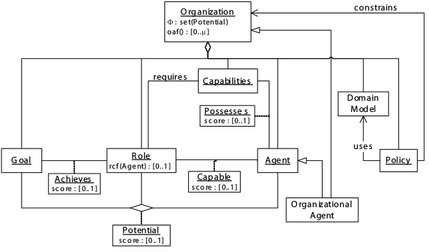
\includegraphics{chapiter1/img/omacs}
	\caption{\label{fig:OMACS meta-models}OMACS meta-models}
\end{figure}

OMACS defines an organization as a tuple O = \textlangle{} G, R, A, C, $\varPhi$ , P, $\sum$ ,
oaf, achieves, requires, possesses \textrangle{}
where
\begin{itemize}

\item[ G ]  
: goals of the organization 
\item[ R ]  
: set of roles  defines a set of roles (i.e., positions within an organization whose behavior
 is expected to achieve a particular goal or set of goals)
\item[ A ]  
: is a set of agents, which can be either human or artificial (hardware or software)
 entities that perceive their environment
\item[ C ]  
: set of capabilities  which define the percepts/actions at their disposal. Capabilities can be soft 
(i.e., algorithms or plans) or hard (i.e., hardware related actions)
\item[  $\varPhi$ ]  
:  relation over G - R - A defining the current set of agent/role/goal assignments
\item[ P ] 
:  set of constraints on  $\varPhi$  formally specifies rules that describe how O OMACS may or may not 
 behave in particular situations
\item[ $\sum$ ]  
: domain model used to specify objects in the environment, their inter-
relationships
%The domain model is a critical component that defines the ontology used to define behavioral policies 
\item[ achieves ]   
: function G $\times$ R $\rightarrow$ {[}0..1{]} a function whose arguments are a goal in G   as well
 as a role in R   that generates an output which is a positive real number greater  than or equal to 0 
 and less than or equal to 1 , defining how effective the behavior
 defined by the role could be in the pursuit of the specified goal   (  the extent of achievement of a goal by a role)
\item[requires] 
: function R $\rightarrow$ P(C)    a function that assumes a role in R  , thereby yielding a set 
of capabilities required to play that role  defining the set of capabilities required to play a role 1
\item[possesses] 
:   function A $\times$ C $\rightarrow$ {[}0..1{]} a function with an agent in A   and a capability in C 
  as inputs yields a positive real number in the range of [0,1] defining the quality of an agent?s capability



\end{itemize}
OMACS also includes two additional derived functions to help compute potential assignment values: 
capable and potential.

\begin{itemize}

\item[capable]   
:	function A $\times$ R $\rightarrow$ {[}0..1{]} function whose inputs are an agent in A OMACS
and a role in R OMACS and generates an output, which is a positive real number greater than or equal to 0 
and less than or equal to 1
defining how well an agent can play a role (computed based on requires and possesses)
\begin{equation}
\begin{cases}
0 & \textrm{if}\prod_{c\subset require(r)}posseses(a,c)=0\\
\frac{\sum_{_{c\subset require(r)}}posseses(a,c) }{|require(r)|} & \textrm{ else}
\end{cases}\label{eq:capable equation}
\end{equation}

\item[potential]
: function A $\times$ R $\times$ G $\rightarrow$ {[}0..1{]}  a function with an agent in A OMACS ,
a role in R   , and a goal in G   as inputs yields a positive real number in the range of {[}0..1{]} ,
thus yielding	
\begin{equation}
potential(a,r,g)=achieves(r,g)\times capable(a,r) \label{eq:potential equation}
\end{equation}
defining how well an agent can play a role to achieve a goal (computed based on capable and achieves)

\item[ OAF ] 
: function ( $ \textrm{G} \times \textrm{R}  \times \textrm{A} $ )  $\rightarrow$ {[}0.. $\infty${]} 
he selection of $\varphi$ from the set of potential assignments is defined by the organization?s reorganization function
, oaf, that assumes a set of assignments in $\varphi$,
thereby yielding a positive real number in the range of {[}0.. $\infty${]}
defining quality of a proposed assignment set
\begin{equation}
OAF=\sum_{(a,r,g)\in\varPhi}potential(a,r,g)\label{eq:oaf equation}
\end{equation}


\end{itemize}

\subsection{Main Element of OMACS}



The first eight elements in the organization tuple defined above G, R, A, C, $\varPhi$ , P, $\sum$  and oaf  constitute the main elements of the OMACS model as depicted in Figure \ref{fig:OMACS meta-models}.

\subsubsection{Goals}

Artificial organizations are designed with a specific purpose, which defines the overall function
of the organization. [2-omacs]

Goals are defined as a desirable situation [37] or the objective of a
computational process .

Within OMACS, each organization has a set of goals, G, that it seeks
to achieve.

OMACS makes no assumptions about these goals except that they can be assigned to
individual agents and individual agents have the ability to achieve them independently . [2-omacs]

\begin{figure}[th]
	\centering
		
\includegraphics{chapiter1/img/Goal}
	\caption{\label{fig:Goal Node}Goal Node }
\end{figure}

\subsubsection{Roles } 

Within OMACS, each organization contains a set of roles (R) that it can use to achieve its goals.
A role defines a position within an organization whose behavior is expected to achieve a
particular goal or set of goals.[2-OMACS]

Thus, each role defines a set of responsibilities. Roles are
analogous to roles played by actors in a play or by members of a typical corporate structure. A
typical corporation has roles such as  president ,  vice-president , and  mail clerk .  

Each role has specific responsibilities, rights and relationships defined in order to help the corporation
perform various functions towards achieving its overall goal. 

Specific people (agents) are assigned to fill those roles and carry out the roles responsibilities using the rights and
relationships defined for that role.[2-OMACS]

OMACS roles consist of a name and a role capability function, rcf. Each role, r $\in$ R, is a tuple
\textlangle{} name, rcf\footnote{the same capable function} \textrangle{}  where A $\times$ R $\rightarrow$ {[}0..1{]} .


The rcf is defined at design time for each role and computed in terms of 
the capabilities required to play that role.
A default rcf (as shown in \ref{eq:capable equation}) 
would assume that all the capabilities required to play a role r are equally important,
essentially taking the average of all the required possesses values (possesses(a,c))
(with the stipulation that none of those possesses scores are 0). [4-OMACS]

\begin{figure}[th]
	\centering
		
\includegraphics{chapiter1/img/Role}
	\caption{\label{fig:Role Node}Role Node }
\end{figure}

\subsubsection{ Agents}

OMACS also includes a set of heterogeneous agents (A) in each organization. 
As described by Russell and Norvig, an agent is an entity that perceives and can perform actions upon its
environment  , which includes humans as well as artificial (hardware or software) entities. [2-OAMCS]

For our purposes, we define agents as computational systems that inhabit some complex dynamic
environment, sense and act autonomously in this environment, and by doing so realize a set of
goals. Thus, we assume that agents exhibit the attributes of autonomy, reactivity, pro-activity, and
social ability. Autonomy is the ability of agents to control their actions and internal state.


Reactivity is an agents ability to perceive its environment and respond to changes in it, whereas
pro-activeness ensures agents do not simply react to their environment, but that they are able to
take the initiative in achieving their goals. 

Finally, social ability allows agents to interact with
other agents, and possibly humans, either directly via communication or indirectly through the
environment.

Within the organization, agents must have the ability to communicate with each other, accept
assignments to play roles that match their capabilities, and work to achieve their assigned goals. [2-OAMCS]

\begin{figure}[th]
	\centering
		
\includegraphics{chapiter1/img/Agent}
	\caption{\label{fig:Agent Node}Agent Node }
\end{figure}

\subsubsection{ Capabilities } 

Capabilities are the key to determining exactly which agents can be assigned to which roles
within the organization. Capabilities are atomic entities used to define a skill or capacity of
agents. [2-OAMCS]

Capabilities can be used to capture soft abilities such as the access to/control over specific
resources, the ability to communicate with other agents, the ability to migrate to a new platform,
or the ability to carry out plans to achieve specific goals. 

Capabilities also capture the notion of hard capabilities that are often associated 
with hardware agents such as robots. 

These hard capabilities are generally described as sensors, which allow the agent to perceive a real world
environment, and effectors, which allow the agent to act upon a real world environment  [2-OAMCS]

\begin{figure}[th]
	\centering
		
\includegraphics{chapiter1/img/Cap}
	\caption{\label{fig:Cap Node}Cap Node }
\end{figure}


\begin{equation}
\forall\textrm{ c : C }\left(\textrm{ a : A c }\in\textrm{possese(a,c) }\geq1\lor\textrm{ r : R c }\in\textrm{requires(r)}\right)\label{eq : capabilities}
\end{equation}


\subsubsection{ The Tuple  $\varphi$ } 
An assignment set $\varphi$ is the set of agent-role-goal tuples  \textlangle{} a,r,g \textrangle{} , that indicate that agent a has been as-signed to play role r in order to achieve goal g .[4-OAMCS]

$\varphi$ is a subset of all the potential assignments of agents to play roles to achieve goals. This set of potential assignments is captured by the potential function (see Equation \ref{eq:potential equation}), which maps each agent-role-goal tuple to a real value ranging from 0 to 1 representing the ability of an agent to play a role in order to achieve a specific goal.
	  
If \textlangle a,r,g \textrangle $\in \varphi$ , then agent a has been assigned by the organization to play role r in order to achieve goal g . [4-OAMCS]

The only inherent constraints on $\varphi$ is that it must contain only assignments whose potential value is greater than zero (Equation \ref{eq:TuplePhi1}) and that only one agent may be assigned to achieve a goal at a time (Equation \ref{eq:TuplePhi2})		


\begin{equation}
\varPhi\subseteq\left\{ \left(\textrm{a,r,g}\right)\brokenvert\textrm{a}\in\textrm{A \ensuremath{\land}}\textrm{r}\in\textrm{R \ensuremath{\land\textrm{g}\in\textrm{G \ensuremath{\land} \textrm{potential(a,r,g) \ensuremath{\ge} 0}}}}\right\} 
\label{eq:TuplePhi1}
\end{equation}

\begin{equation}
\forall\textrm{a1,a2:A r1,r2:R g1,g2:G (a1,r1,g1)}\in\varPhi\land\textrm{(a2 r2 g2)}\in\varPhi\land\textrm{a1=a2}\label{eq:TuplePhi2}
\end{equation}

 		
 

\subsubsection{ OAF }
	In order to select the best set of assignments to maximize an organizations ability to achieve its goals, OMACS defines an organizational assignment function, or oaf , which is a function over the current assignment set, oaf: $\varphi$ $\rightarrow$ 0..$\infty$. As with the rcf , the selection of assignments may be application specific. [4-OMACS]
	
Thus, each organization has its own application specific organization assignment function, oaf , which computes the goodness of the organization based on $\varphi$. 
	
As with the rcf , we can define a default  oaf , which is simply the sum of the potential scores in the current assignment set $\varphi$.
                     
 
\subsubsection{ Domain Model } 

The domain model, $\sum$, is used to define object types in the environment 
and the relations between those types. [2-OMACS]

The domain model is based on traditional object oriented class diagrams. They
include object classes that each have a set of attribute types. 

Relations between object classes include general purpose associations
 as well as generalization-specialization and aggregation.
 
Relations may also include multiplicities to constrain the number of object classes participating in
any given relation.[2-OMACS]
 





%\bigskip 

 
\subsection{ Function of OMACS }

There are three major relations/functions and two derived functions between the eight main elements that provide the power of the OAMCS model: achieves, requires, possesses, capable, and potential. 
\subsubsection{The Achieves}
function (although somewhat confusingly named) actually defines how effective an agent could be while playing that role in the pursuit of a specific goal. For instance, if one role requires more resources or better capabilities, it can use a different approach and thus yield better results than a second role that requires fewer resources or capabilities. [4-OMACS]

 Providing two different roles to achieve the same goal  may provide the organization flexibility in deciding how to actually achieve a given goal.

 The value of achieves can be predefined by the organization designer or learned before or during system operation (Odell, Nodine \& Levy, 2005). Thus, the OMACS achieves function formally captures the effective- ness of a role in achieving a specific goal by defining a total function from the R $\times$ G to a real value in the range of 0 to 1, achieves: G $\times$ R $\rightarrow$ {[}0..1{]}.
 
  Thus, by definition, a role that cannot be used to achieve a particular goal must have an achieves value of 0, while a role that can achieve a goal would have an achieves value greater than zero.[4-OMACS]

\begin{figure}[th]
	\centering
		\includegraphics{chapiter1/img/a}
	\caption{\label{fig:The Achivement Relation}The Achivement Relation }
\end{figure}
 

\subsubsection{Requires}

In order to perform a particular role, agents must possess a sufficient set of capabilities that allow
the agent to carry out the role and achieve its assigned goals. [2-OMACS]

For instance, to play the  president role,
 a person would be expected to have knowledge of the corporations domain, experience in
lower-level jobs in similar types of companies, and experience in managing people and resources;
an artificial organization is no different. 

Roles require a certain set of capabilities while agents
possess a set of capabilities [2-OMACS]


\begin{figure}[th]
	\centering
		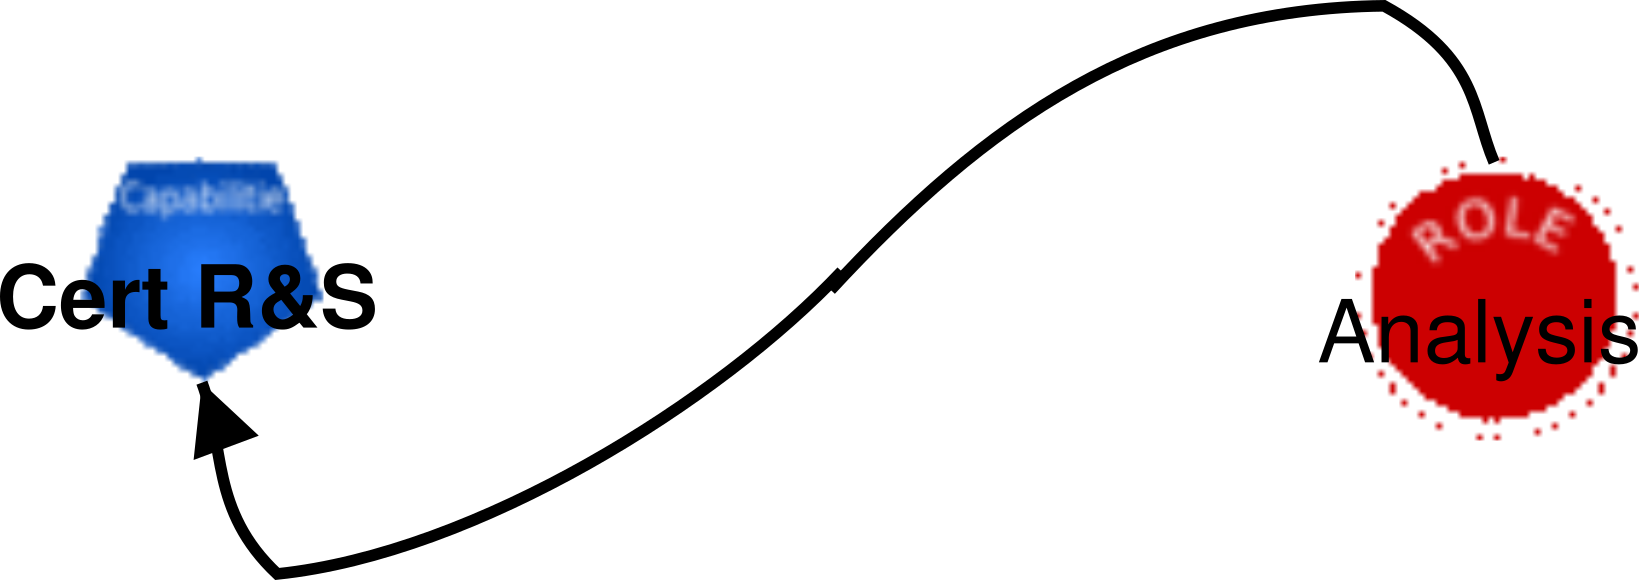
\includegraphics{chapiter1/img/r}
	\caption{\label{fig:The Requirment Relation}The Requirment Relation }
\end{figure}



\subsubsection{Possesses}
In order to determine if some agent has the appropriate set of capabilities to play a given role, OMACS defines a similar relation, the possesses relation, that captures the capabilities a specific agents actually possesses. [4-OMACS]

The possesses relation is formally captured as a function over agents and capabilities that returns a value in the range of 0 to 1,

 possesses: A $\times$ C $\rightarrow$ [0..1]. The real value returned by the possesses function indicates the quality of each capability possessed by the agent; 0 indicates no capability while a 1 indicates a high quality capability. [4-OMACS]


\begin{figure}[th]
	\centering
		
\includegraphics{chapiter1/img/p}
	\caption{\label{fig:Possesses Relation}Possesses Relation }
\end{figure}


\subsubsection{Capable}
Using the capabilities required by a particular role and capabilities possessed by a given agent, we can compute the ability of an agent to play a given role, which we capture in the capable function. The capable function returns a value from 0 to 1 based on how well a given agent may play a specific role, capable: A $\times$ R $\rightarrow$ {[}0..1{]} . [2-OMACS]

Since the capability of an agent, a, to play a specific role  r , application and role specific, OMACS provides the rcf defined in the previous section that controls how this value is computed. Thus, the capable score of an agent playing a particular role is defined via the designer defined rcf of each role.
%#houssam  equation1
\begin{equation}
\forall a:A\textrm{ r:R }capable(a,r)=r.rcf(a)\label{eq:Funccapable}
\end{equation}
While the rcf is user defined, it must conform to one OMACS constraint. 
To be capable of playing a given role in the current organization,
 an agent must possess all the capabilities that are required by that role . [2-OMACS]
%equation2 
\begin{equation}
\text{\ensuremath{\forall}}a:A,r:Rcapable(a,r)>0\text{\ensuremath{\Leftrightarrow}}requires(r)\text{\ensuremath{\subseteq}}{c|possesses(a,c)>0}\label{eq:FuncCapable2}
\end{equation}



\begin{figure}[th]
	\centering
		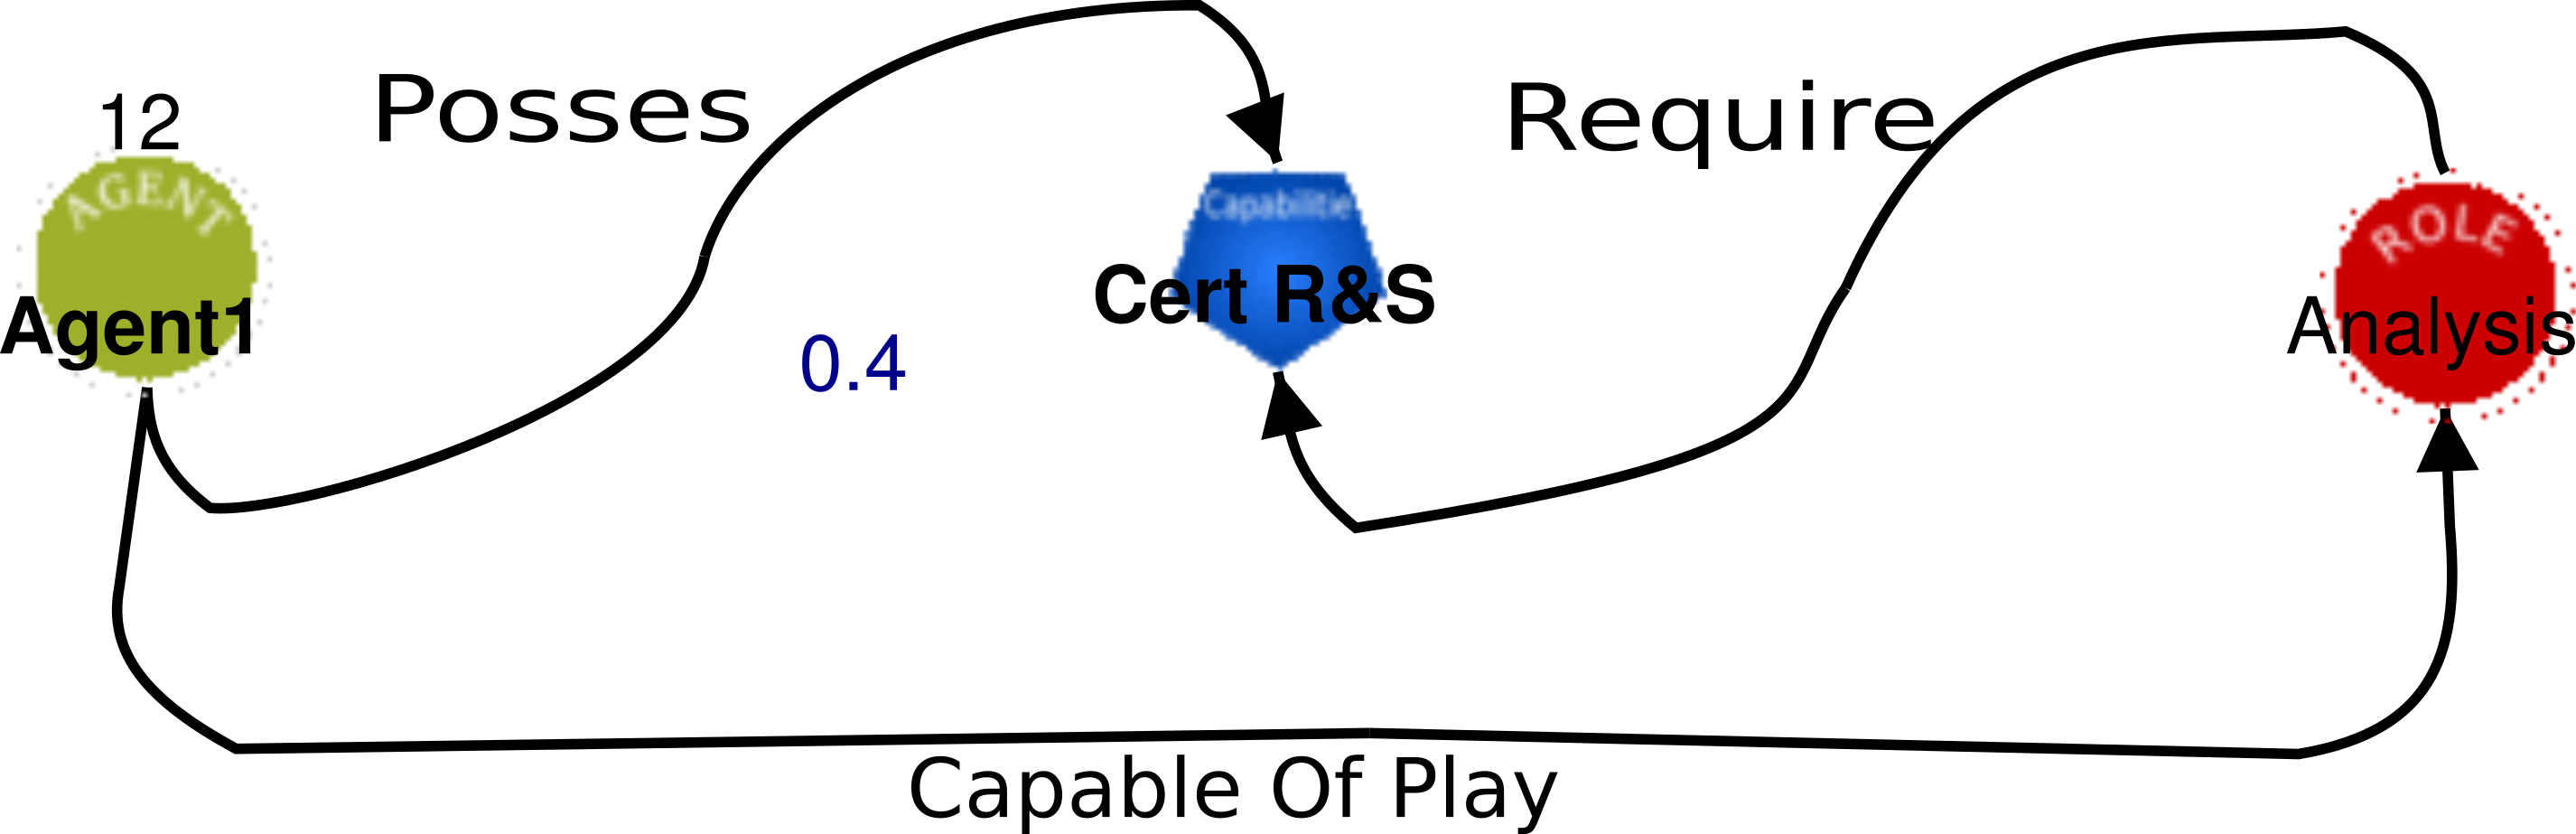
\includegraphics{chapiter1/img/c}
	\caption{\label{fig:Capable Of playing Relation} Agent Capable of Playing Analysis Role}
\end{figure}

\pagebreak


The main goal of OMACS is to provide a mechanism to assign goals to agents [2-OMACS]

in such a way that agents cooperate toward achieving some top-level goal.
Intuitively, this mechanism should provide a way to assign the best agents 
to play the best roles in order to achieve these goals. 

Thus, OMACS has defined  a potential function that captures the ability of an agent 
to play a role in order  to achieve a specific goal.   [2-OMACS]


\subsubsection{Potential}
The potential function maps each agent-role-goal tuple to a real value ranging from 0 to 1, 
potential: A $\times$ R $\times$ G $\rightarrow$ [0..1].[4-OMACS]

Here, a 0 indicates that the agent-role-goal tuple cannot be
used to achieve the goal while a non-zero value indicates how well an agent can play
a specific role in order to achieve a goal.  

The potential of agent a to play role r 
to achieve goal g is defined by combining the capable and achieves functions.[4-OMACS]

\begin{equation}
\forall a:A\textrm{ r:R g:G }potential(a,r,g)=achieves(r,g)*capable(a,r)\label{eq:potentialFunc}
\end{equation}







































%this section should you read it more and reOrgnize 
\section{ Organization \& Reorganization Dynamic System}
 
The constraints above define the legality of the organization structure and its instances.  However,we are also interested in whether or not an assignment of agents to roles satisfying all the organizational policies exists that can allow the system to achieve its goals, which we refer to as organizational viability. [2-OMACS]

Although an organization may be structurally valid, there is no guarantee that an instance of that organization exists that can achieve its goals. 

In actuality, we can never guarantee that the system will ever achieve all its goals due to the dynamic nature of the environment in which the organization operates. To achieve the organizational goals, the system must have the right mix of agents to play the right roles to achieve those goals. 

Essentially, a viable organization is a valid organization that has been populated with the right types and numbers of agents so that it might potentially achieve its goals. [2-OMACS]

\subsection{ Organization and Reorganization }
Each organization has an implicitly defined organization transition function 
that describes how the organization may transition from one organizational state 
to another over the lifetime of the organization.  [2-OMACS]
	
Since agents in an organization as well as their individual capabilities may change over time, 
this function cannot be predefined, but must be computed based on the current state, 
the goal set, G, and the current policies. In our present research with purely autonomous systems, we have only considered reorganization that involves the state of the organization. 

However, we have defined two distinct types of reorganization: state reorganization, which only allows the modification of the organization state, and structure reorganization, which allows modification  of the organization structure (and may require state reorganization to keep the organization consistent).

We define the state of the organization as the set of agents, A, the possesses, capable, and potential functions, and the assignment set, $\varphi$. However, not all these components may actually be under the control of the organization. For our purposes, we assume that agents may enter or leave organizations or relationships, but that these actions are triggers that cause reorganizations and are not the result of reorganizations. 

Likewise, possesses (and thus capable and potential as well) is an automatic calculation that determines the possible assignments of agents to roles and goals in the organization. The calculation of possesses is the only calculation totally controlled by the agent; the organization can only use this information in deciding how to make assignments. This leaves one element that can be modified via state reorganization: $\varphi$.
	[2-OMACS]
\subsubsection{ Goal Set Changes }
Any change in G may cause reorganization. There are three basic types 
of events that can cause achange in G: 
\begin{enumerate}
\item   insertion of a new goal  
\item   goal achievement 
\item   goal failure
\end{enumerate}

is discussed below. 

The first situation deals with new goals being added to G. However, [2-OMACS]
we cannot say with certainty that reorganization will occur based on a new goal in G. 

It is possible that the organization will choose to forego reorganization for a number of reasons, the most likely being that it has simply chosen not to pursue any new goals added to G at the present time.

The second case deals with goal achievement. When a goal g is achieved, G is changed to reflect that event by 

\begin{itemize}
\item  removing g from G
\item  possibly adding new goals
\end{itemize}	

 which are enabled by the achievement of g, into G. Obviously, the agent assigned to achieve goal g is now free to pursue other goals. 

The third instance involves goal failure, which really has two forms: agent-goal failure and goal failure.

When a specific agent cannot achieve goal g but g might still be achievable by some other agent, 
agent-goal failure occurs. 

When agent-goal failure occurs, reorganization must occur to allow the organization to 

\begin{itemize}
\item  choose another agent to achieve g
\item  not pursue g at the current time
\item  choose another goal to pursue instead of g
\end{itemize}	
 
In any of these situations, g is not removed from G since it has not been achieved. In the case where the organization or the environment has changed such that a goal g can never be achieved, then goal failure occurs. 

In this case, g is removed from G and the organization must attempt to assess whether it can still achieve the overall system goals. Reorganization may occur to see if the agent assigned to achieve g can be used elsewhere. 

In all cases, the selection of the appropriate strategy is left to the organization. [2-OMACS]

\subsubsection{Agent Changes }
The second type of change that triggers reorganizations are changes to the set of agents, A, or their individual capabilities.[2-OMACS]

When an agent that is part of $\varphi$ is removed from the organization, a reorganization must occur, even if only to remove the agent and its assignment(s) in $\varphi$. Likewise,when an agent that is part of $\varphi$ loses a capability that negates its ability to play a role that it is assigned, reorganization must occur as well. 

In general, when changes occur in an agent?s capability, reorganization may or may not be necessary, based on the agents capable relation. 

We have identified four specific types of changes in an agents capabilities that may indicate a need for reorganization: 

\begin{enumerate}
\item 
	when an agent gains the ability to play a new role
\item
	when an agent loses the ability to play a role
\item
	when an agent increases its ability to play a specific role
\item
	when an agent decreases its ability to play a specific role.
\end{enumerate}	
 
While case 2 requires reorganization if the agent is currently assigned to play the role for which it no longer has the capability to play, whether or not to reorganize is left up to theorganization when the other three cases (along with 2 when the agent is not currently assigned that role) occur. [2-OMACS]


\subsection{ Reorganization }
Reorganization is the process of changing the assignments of agents to roles to goals as specified
in $\varphi$.  [2-OMACS]

The organization?s oaf function is used to determine the best new $\varphi$; however, total
reorganization may not be necessary or efficient. (In the absence of any information or policies,
an optimal total reorganization would take on the order of 2 A$\times$G$\times$R .)

One approach is to take a local view, in which the organization looks at the OMACS state and
reorganizes in a locally optimal fashion (i.e. hill climbing).
However, when dealing with dynamic environments, it is often desirable to reorganize so that 
the team can operate more efficiently or
effectively in its present situation as well as being adaptable to its changing environment. 

Thus, we would like to take a long-range or global view. Unfortunately, it has been shown that in the
general case globally optimal reorganizations are NEXP-complete and, thus impractical for most
applications with any time constraints . 

Therefore, OMACS provides a mechanism for augmenting the locally optimal algorithm with application specific rules in an attempt to make
reasoning more efficient and to enable globally better solutions.
[2-OMACS]
\subsubsection{ General Purpose Reorganization Examples }

For general-purpose reorganization, the Developers have developed several reorganization algorithms that
give us a default reorganization capability. When a reorganization trigger occurs, general-purpose
reorganization algorithms can be used to find appropriate assignments to achieve the
organizations goals, if possible. [2-OMACS]

To compute the best reorganization, an algorithm that simply
optimizes the organizations oaf might seem appropriate; however, this approach is short sighted.
First, it does not deal with the cost associated with reorganizing and, second, it does not consider
the reason reorganizing was initially undertaken. Exploiting reorganizing costs requires a
distributed solution since the cost for robots to change roles is not globally known. 

For instance, if an agent is required to perform a complex computation, any effort toward that computation
would be lost if the agent was reassigned to another role/goal Considering the reason for
reorganization may enable less extensive (and less costly) reorganization. If the reason for
reorganizing is to fill a single role, then a total reorganization may be a waste of time and
resources. [2-OMACS]

\pagebreak

\section{Conclusion}

This chapter describes how to design adaptive multiagent
systems using an organizational model, which defines the
entities and relationships of a typical organization.

 The major elements of the model consist of goals, roles, agents,
capabilities, and the relationships between them. By
designing a system using the model, and we focus on OMACS framework
because it handeling reorganization system more then other framework

In the following chapter will discuss other model
we can use it to modeling the multi-Agent System
\textbf{}


%
\chapter{\label{cha:pgraph}PGraph and PNS}

 
In a process system , raw materials are consumed through various transformation to yield desired products . 
This is usually accompanied bu the generation of wastes .Vassels in which these transformations are carried out are termed operating units of the process , a given set of operating units with the plausible interconnections can be described bu a network The desired products can often be manufactured using some sub networks of this network , thus a given network may give rise to a variety of processes producing the desired products , and each of such process corresponds to sub network which can be considered  to be its structure
\section{ PGraph }


The so called P graph (Process graph), which is a directed bigraph, has been used for modelling network structures for some time.
The vertices of the graph denote the operating units (O   operating units) and the materials (M   materials).
The edges of the graph represent the material-flow between the materials and the operating units.
\subsection{ General Definition of P-Graph }

The Pgraph is a bigraph, meaning that its vertices are in disjunctive sets and there are no edges between vertices in the same set.
In case of P graphs the assignment of operating units and materials are strictly determined by the tasks given, i.e. an edge can point to an M material type vertex from an O operating unit type vertex, only if M is element of the output set of O, that is O produces M material namely, M $\in$ output O . 


An edge can point from an M material type vertex to an O operating unit type vertex, only if M is element of the input set of O, that is O processes M material, namely M  $\in$ input O. .
Thus, the P-graph can be presented by the pairs of operating unit and the assigned material vertices set like the (M,O) P-graph.
The material type vertices can be put into several subsets. 
There are various subsets like the raw-material type one, which contains the input elements of the whole process, the product-material type subset, which gathers the results of the entire process, the intermediate-material type one, the elements of which emerge or are used between the processing phases, and finally the by-product-material  type set, which contains the non desired results of the process. The applied operating unit and material element notations in the P-graph notation are presented in \ref{fig:example for P-graph}.

As an example let us consider a process network with 7 operating units, in which the operating units are 1,2....7 and the materials are A,B, .... L. A,B,C and D are the materials available for the production of L The possible structure is given in  .

\begin{figure}[th]
	\centering
		\includegraphics{chapiter2/img/notationP}
	\caption{\label{fig:notation in pgraph}notation in pgraph}
\end{figure}


\begin{figure}[th]
	\centering
		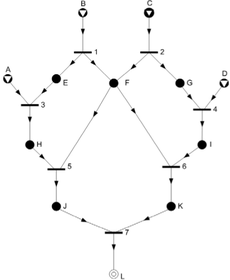
\includegraphics{chapiter2/img/examplePgraph}
	\caption{\label{fig:example for P-graph}example for P-graph }
\end{figure}

\section{ Process Network Synthesis }

In the Process Network Synthesis (PNS for short) problem a set of materials is given and also operating units 
which are transforming some subset of materials into some other subset.
The subsets assigned to the operating unit are called its  input and output materials. 
In the problem two subsets of the materials are distinguished, 
one is the set of the raw materials and the other is the set of the desired products.
Our goal is to find a minimal cost network of the operating units which can produce all desired products starting from the raw material. These systems can be modeled in the P-graph framework which is based on bipartite graphs.


In these P-graphs we have two sets of vertices, one of them contains the possible materials,
the other the operating units. The edges lead to an operating unit from its input materials 
and from an operating unit to its output materials. 


Then the subgraphs satisfying some properties describe the feasible processes
which produce the desired products from the raw materials.
Thus our goal is to find the least expensive such subgraph. 
In the structural model the amounts of the material flows are not taken into account thus the cost of an operating unit is a constant, and the cost of a subgraph is the sum of the costs of the operating units contained in it. 
\subsection{ Basic Notation }

The structural PNS problem can be modeled in the PGraph framework.
In the PGraph (Process Graph) we have the set of the materials denoted by M,
which contain two special subsets, the set of raw materials and the set of desired products denoted by R and P respectively

The problem also contains a set of possible operating units which can transform some sets of materials. 

The set of operating units is denoted by O. An operating unit u is given by two sets, 
in(u) denotes the set of the input materials out(u) denotes the set of output materials of the operating unit

This means that the operating unit can work in a solution structure if all of its input materials are produced and in this case it 
produces all of its output materials. 

The PGraph  of the problem is defined by the sets M and O. It is a directed bipartite graph where the set of vertices is M $\cup$ O, and have the following two sets of edges:
\begin{enumerate}
\item Edges which connect the input materials to their operating unit
\item Edges which connect the operating units to their output materials
\end{enumerate}

Then some of the subgraphs of this P-graph describe the feasible solutions which produce the required materials from the raw materials.  
where m and o are the subsets of M and O, represent a feasible solution if and only if the following properties called axioms are valid: 
\begin{enumerate}

\item m contain all element of P    
\item a material from m is a raw material if and only if no edge goes into it in the P-graph (m, o)  
\item For each operating unit u from o there exists a path in the P-graph (m,o) which goes into a desired product from u  
\item m is the union of the input and output material sets of the operating units contained 
in set o  
 
\end{enumerate}

\subsection{Mathematical definition }

There is a finite set of material M (which contains the sets of P products and R raw-materials) 
and the finite set of O operating units. 
Consequently, the set of P end-products and the set of R raw-materials must be subsets of M 
and the set of M materials and the set of O operating units are disjunctive.
The basic relations between M,P,R and O are as follows : 

\begin{equation}
P\subseteq M,R\subseteq M,M\cup O=\emptyset\label{eq:1}
\end{equation}

As physical processes are defined, each operation unit produces output materials from
input materials. Therefore two disjunctive sets can be assigned to each operating unit, i.e. the set of input and the set of output materials. 

Let an arbitrary operating unit ( $\alpha$ , $\beta$), then $\alpha$ is the set of input materials which are processed by the 
($\alpha$ , $\beta$ ) unit and $\beta$is the set of output materials, which are produced by the given unit .


Considering the process-network the output materials of each operating unit are the inputs of different operating units. In general, it can be proved that 

\begin{equation}
O\subseteq \rho(M) \times  \rho(M)\label{eq:second}
\end{equation}

where O is the set of operating units, M is the set of materials and $\rho(M)$ is the power set, 
that is the set of subsets of M, and $\rho(M) \times  \rho(M)$ represents the set of $\rho(M)$ and $\rho(M)$ pairs

Supposing that there is a finite set m, which is a subset of M, i.e. it is true that m $\subseteq$ M 
and there is an o finite set, which is a subset of O, i.e. 
it is true that o $\subseteq$ O and supposing that there is such a material
which is an input for one or more operating units, and there is such material 
which is the output of one or more operating units, then :

\begin{equation}
o\subseteq \rho(m) \times  \rho(m)\label{eq:second}
\end{equation}


The PNS is defined as a bigraph, where the set of V vertices is made of the elements of the union of m and o that is

\begin{equation}
V = m \cup o\label{eq:nex}
\end{equation}
 
 

\subsection{ Algorithms MSG, SSG, and ABB }
PNS representation of a process network and the set of  axioms for solution structures, i.e.,
combinatorial feasible networks, render it possible to fashion the three mathematically rigorous algorithms:
MSG, SSG, and ABB. 

The algorithm MSG (Maximal-Structure Generation) generates the maximal structure (super-structure)
of a process synthesis network.
Also, 

the algorithm SSG (Solution-Structure Generation) generates the set of feasible process structures from the maximal structure,

which leads to the algorithm ABB (Accelerated Branch and Bound) for computing the n-best optimal solution structure
\subsubsection{Maximal-Structure Generation}
The maximal structure of the synthesis problem (P, R, O) contains all the combinatorially possible structures, which make the production of defined products possible from given raw-materials. Therefore, it certainly contains the optimal structure as well.

The first phase is the input phase, in which the synthesis problem is defined (P, R, O) such a way, that the set of M all the plausible materials, the set of P end-products 

The second phase is the elaboration of the input structure of the network, which is carried out by the linking of all the similar (same type) material type vertices.

The third phase is the elimination phase, where those materials and operating units are eliminated, which, taking the  axioms into account, are not and cannot be linked to the maximal structure for sure

During the fourth phase the vertices are linked again from level to level, starting from the highest, the end-product level.

The maximal structure generated this way contains all the combinatorially possible structures and all of its elements fulfil the  axioms.
\subsubsection{Maximal-Structure Generation}
The maximal structure generated by the MSG algorithm contains all such combinatorically possible network structures that are able to produce the end-product from the given raw-materials.

Consequently, it contains the optimal network as well. In most cases the optimalisation means to find the most cost effective solution.

The application of the SSG (Solution Structure Generation) algorithm enables the production of all the solution structures. The SSG is a new mathematical tool  which has been developed by Friedler et al.

\subsubsection{Accelerated Branch and Bound}

The branch-and-bound method has been widely used The method is reiterated here to facilitate formalization of the
accelerated branch-and-bound algorithm of PNS.
to Identify the optimal process from the maximal structure 


\subsection{ Comparaison PNS and PetriNet : }
\begin {table}[H] 
\begin{tabular}{cc}

\hline 
\textbf{Petri Net}  & \textbf{Process Network Synthesis}\tabularnewline
\hline 
Source Place  & Raw Material\tabularnewline
Normal Place  & Intermediate Material\tabularnewline
Sink Place  & Final Product\tabularnewline
Token in Place  & Requirement Flow \tabularnewline
Transition  & Operating Unit \tabularnewline
Weight of in or out edges of the  transition & producing rate of the operating unit\tabularnewline
\hline 
Modeling Parallel System  & Basically use for Chemical Reaction \tabularnewline
\hline 

\end{tabular}
\caption {Petri Net and PNS}
 
\end {table}

\section{Conclusion}
in this chapter , i presente the definition of second framework i use
PGraph and define the Process Network synthesis .
with some Algorithme applicable on PNS
to find the optimum structure

%
\chapter{\label{cha:org}Organization Multi-Agent System}

Designing and implementing large, complex, and distributed systems by resorting to autonomous 
or semi-autonomous agents that can reorganize themselves by  cooperating with one another 
represent the future of software systems   A set of  methodologies  a selection of design processes ,
and a collection of  frameworks are available in the literature to provide the basis for constructing 
sophisticated autonomous multi-agent organizations . [0-omacs]
 
 
Moreover, a set of metrics and methods have been suggested with the intention of providing useful information 
about key properties (e.g., complexity, flexibility, self-organized, performance, scalability, and cost)
of these multi-agent organizations  .[0-omacs]

This chapter introduces a suite of technologies for building complex, adaptive systems. 
It is based in the multi-agent systems paradigm and uses the Organization Model for Adaptive 
Computational Systems  (OMACS). 
And presents a suite of technologies including  the Organization-based Multiagent Systems Engineering 
(O-MaSE) methodology [4-omacs]

\section*{ \Huge{Framework of Modilization MaS} }
\section{ Organization Multi-Agent System Engineering}
\subsection{ Overview of O-MaSE }
 the Organization-based Multiagent System Engineering (O-MaSE) is a framework that 
 allows designers to create custom agent-oriented development processes. 
 
This custom agent-oriented process is generated following a process metamodel 
and then instantiated from a set of method fragments and guidelines 
by using a method engineering approach . 

O-MaSE defines a metamodel, a repository of method fragments and a set of guidelines. 
The O-MaSE metamodel defines general concepts used in multiagent systems
along with their relationships and is based on an organizational approach. [6-omacs]
 
The O-MaSE Process Framework is based on the OPEN Process Framework (OPF)
 and uses the OPF metamodel  , as shown in Figure \ref{fig:O-MaSE Process Framework}  .[4-omacs]

\begin{enumerate}
\item 
	level M2 : which defines processes in terms of Work Units (Activities, Tasks, and Techniques),
	 Producers, and Work Products.
\item
	Level M1 : contains the definition of O-MaSE in the form of the O-MaSE metamodel, method fragments
	, and guidelines. 
\item
	Level M0  : level for specific projects (a process instance).
\end{enumerate} 

\begin{figure}[th]
	\centering
		\includegraphics{chapiter1/img/omase}
	\caption{\label{fig:O-MaSE Process Framework}O-MaSE Process Framework}
\end{figure}
\subsection{ The Goal of O-MaSE }

The goal of the O-MaSE methodology framework is to allow method engineers to
build custom agent-oriented methods using a set of method fragments, all of which are
based on a common meta-model. [7-omacs]

To achieve this, O-MaSE is defined in terms of a meta-model, a set of method fragments, and a set of method construction guidelines. 

The O-MaSE meta-model defines a set of analysis, design, and implementation concepts and a
set of constraints between them. 

The method fragments define a set of work products, a set of activities that produce work products, and the performers of those activities.

And the method construction guidelines define how the method fragments may be
combined to create O-MaSE compliant methods

The O-MaSE methodology is supported by the agentTool III \footnote{http://agenttool.cs.ksu.edu/}
 development environment 2 , 
which is designed as a set of Eclipse plug-ins. agentTool includes a plug-in for each O-MaSE model 
and the agentTool Process Editor (APE), which was developed to support the design and definition 
of O-MaSE compliant processes. [7-omacs]

The APE plug-in is based on the Eclipse Process Framework and provides a process designer the ability to : 
\begin{enumerate}
\item 
	extend O-MaSE with new tasks, models, or usage guidelines
\item
	create new process instances by composing tasks
, models, and producers from the O-MaSE method fragment library  
\item
	 verifying that they meet process guidelines
\end{enumerate} 
 
\section{  Organization Model for Adaptive Computational System }
\subsection{ Overview of OMACS }
The OMACS is Framework , this model grew from the MaSE metamodel , 
which was based on the original AGR\footnote{Agent Group Roles}  model . [4-omacs]

We realized that while we could define multiagent systems in terms of agent
playing roles in order to achieve system goals, we did not have to limit the flexibility
of agents by predefining the roles they could and could not play. [4-omacs]

Noting that agents could be assigned to roles based on the capabilities 
Required to play various roles and the capabilities possessed by the agents,
we figured the agents could adapt their assignments based on the current 
set of goals required to be achieved by the system.
This basic idea led to the OMACS  model as defined in DeLoach,
Oyenan, and Matson (2007) and shown in Figure \ref{fig:OMACS meta-models} . [4-omacs]

\begin{figure}[th]
	\centering
		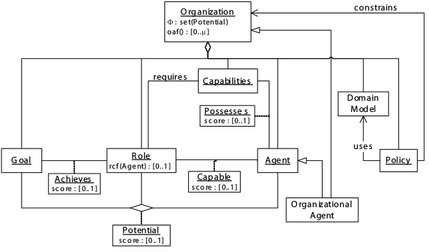
\includegraphics{chapiter1/img/omacs}
	\caption{\label{fig:OMACS meta-models}OMACS meta-models}
\end{figure}

OMACS defines an organization as a tuple O = \textlangle{} G, R, A, C, $\varPhi$ , P, $\sum$ ,
oaf, achieves, requires, possesses \textrangle{}
where
\begin{itemize}

\item[ G ]  
: goals of the organization 
\item[ R ]  
: set of roles  defines a set of roles (i.e., positions within an organization whose behavior
 is expected to achieve a particular goal or set of goals)
\item[ A ]  
: is a set of agents, which can be either human or artificial (hardware or software)
 entities that perceive their environment
\item[ C ]  
: set of capabilities  which define the percepts/actions at their disposal. Capabilities can be soft 
(i.e., algorithms or plans) or hard (i.e., hardware related actions)
\item[  $\varPhi$ ]  
:  relation over G - R - A defining the current set of agent/role/goal assignments
\item[ P ] 
:  set of constraints on  $\varPhi$  formally specifies rules that describe how O OMACS may or may not 
 behave in particular situations
\item[ $\sum$ ]  
: domain model used to specify objects in the environment, their inter-
relationships
%The domain model is a critical component that defines the ontology used to define behavioral policies 
\item[ achieves ]   
: function G $\times$ R $\rightarrow$ {[}0..1{]} a function whose arguments are a goal in G   as well
 as a role in R   that generates an output which is a positive real number greater  than or equal to 0 
 and less than or equal to 1 , defining how effective the behavior
 defined by the role could be in the pursuit of the specified goal   (  the extent of achievement of a goal by a role)
\item[requires] 
: function R $\rightarrow$ P(C)    a function that assumes a role in R  , thereby yielding a set 
of capabilities required to play that role  defining the set of capabilities required to play a role 1
\item[possesses] 
:   function A $\times$ C $\rightarrow$ {[}0..1{]} a function with an agent in A   and a capability in C 
  as inputs yields a positive real number in the range of [0,1] defining the quality of an agent?s capability



\end{itemize}
OMACS also includes two additional derived functions to help compute potential assignment values: 
capable and potential.

\begin{itemize}

\item[capable]   
:	function A $\times$ R $\rightarrow$ {[}0..1{]} function whose inputs are an agent in A OMACS
and a role in R OMACS and generates an output, which is a positive real number greater than or equal to 0 
and less than or equal to 1
defining how well an agent can play a role (computed based on requires and possesses)
\begin{equation}
\begin{cases}
0 & \textrm{if}\prod_{c\subset require(r)}posseses(a,c)=0\\
\frac{\sum_{_{c\subset require(r)}}posseses(a,c) }{|require(r)|} & \textrm{ else}
\end{cases}\label{eq:capable equation}
\end{equation}

\item[potential]
: function A $\times$ R $\times$ G $\rightarrow$ {[}0..1{]}  a function with an agent in A OMACS ,
a role in R   , and a goal in G   as inputs yields a positive real number in the range of {[}0..1{]} ,
thus yielding	
\begin{equation}
potential(a,r,g)=achieves(r,g)\times capable(a,r) \label{eq:potential equation}
\end{equation}
defining how well an agent can play a role to achieve a goal (computed based on capable and achieves)

\item[ OAF ] 
: function ( $ \textrm{G} \times \textrm{R}  \times \textrm{A} $ )  $\rightarrow$ {[}0.. $\infty${]} 
he selection of $\varphi$ from the set of potential assignments is defined by the organization?s reorganization function
, oaf, that assumes a set of assignments in $\varphi$,
thereby yielding a positive real number in the range of {[}0.. $\infty${]}
defining quality of a proposed assignment set
\begin{equation}
OAF=\sum_{(a,r,g)\in\varPhi}potential(a,r,g)\label{eq:oaf equation}
\end{equation}


\end{itemize}

\subsection{Main Element of OMACS}



The first eight elements in the organization tuple defined above G, R, A, C, $\varPhi$ , P, $\sum$  and oaf  constitute the main elements of the OMACS model as depicted in Figure \ref{fig:OMACS meta-models}.

\subsubsection{Goals}

Artificial organizations are designed with a specific purpose, which defines the overall function
of the organization. [2-omacs]

Goals are defined as a desirable situation [37] or the objective of a
computational process .

Within OMACS, each organization has a set of goals, G, that it seeks
to achieve.

OMACS makes no assumptions about these goals except that they can be assigned to
individual agents and individual agents have the ability to achieve them independently . [2-omacs]

\begin{figure}[th]
	\centering
		
\includegraphics{chapiter1/img/Goal}
	\caption{\label{fig:Goal Node}Goal Node }
\end{figure}

\subsubsection{Roles } 

Within OMACS, each organization contains a set of roles (R) that it can use to achieve its goals.
A role defines a position within an organization whose behavior is expected to achieve a
particular goal or set of goals.[2-OMACS]

Thus, each role defines a set of responsibilities. Roles are
analogous to roles played by actors in a play or by members of a typical corporate structure. A
typical corporation has roles such as  president ,  vice-president , and  mail clerk .  

Each role has specific responsibilities, rights and relationships defined in order to help the corporation
perform various functions towards achieving its overall goal. 

Specific people (agents) are assigned to fill those roles and carry out the roles responsibilities using the rights and
relationships defined for that role.[2-OMACS]

OMACS roles consist of a name and a role capability function, rcf. Each role, r $\in$ R, is a tuple
\textlangle{} name, rcf\footnote{the same capable function} \textrangle{}  where A $\times$ R $\rightarrow$ {[}0..1{]} .


The rcf is defined at design time for each role and computed in terms of 
the capabilities required to play that role.
A default rcf (as shown in \ref{eq:capable equation}) 
would assume that all the capabilities required to play a role r are equally important,
essentially taking the average of all the required possesses values (possesses(a,c))
(with the stipulation that none of those possesses scores are 0). [4-OMACS]

\begin{figure}[th]
	\centering
		
\includegraphics{chapiter1/img/Role}
	\caption{\label{fig:Role Node}Role Node }
\end{figure}

\subsubsection{ Agents}

OMACS also includes a set of heterogeneous agents (A) in each organization. 
As described by Russell and Norvig, an agent is an entity that perceives and can perform actions upon its
environment  , which includes humans as well as artificial (hardware or software) entities. [2-OAMCS]

For our purposes, we define agents as computational systems that inhabit some complex dynamic
environment, sense and act autonomously in this environment, and by doing so realize a set of
goals. Thus, we assume that agents exhibit the attributes of autonomy, reactivity, pro-activity, and
social ability. Autonomy is the ability of agents to control their actions and internal state.


Reactivity is an agents ability to perceive its environment and respond to changes in it, whereas
pro-activeness ensures agents do not simply react to their environment, but that they are able to
take the initiative in achieving their goals. 

Finally, social ability allows agents to interact with
other agents, and possibly humans, either directly via communication or indirectly through the
environment.

Within the organization, agents must have the ability to communicate with each other, accept
assignments to play roles that match their capabilities, and work to achieve their assigned goals. [2-OAMCS]

\begin{figure}[th]
	\centering
		
\includegraphics{chapiter1/img/Agent}
	\caption{\label{fig:Agent Node}Agent Node }
\end{figure}

\subsubsection{ Capabilities } 

Capabilities are the key to determining exactly which agents can be assigned to which roles
within the organization. Capabilities are atomic entities used to define a skill or capacity of
agents. [2-OAMCS]

Capabilities can be used to capture soft abilities such as the access to/control over specific
resources, the ability to communicate with other agents, the ability to migrate to a new platform,
or the ability to carry out plans to achieve specific goals. 

Capabilities also capture the notion of hard capabilities that are often associated 
with hardware agents such as robots. 

These hard capabilities are generally described as sensors, which allow the agent to perceive a real world
environment, and effectors, which allow the agent to act upon a real world environment  [2-OAMCS]

\begin{figure}[th]
	\centering
		
\includegraphics{chapiter1/img/Cap}
	\caption{\label{fig:Cap Node}Cap Node }
\end{figure}


\begin{equation}
\forall\textrm{ c : C }\left(\textrm{ a : A c }\in\textrm{possese(a,c) }\geq1\lor\textrm{ r : R c }\in\textrm{requires(r)}\right)\label{eq : capabilities}
\end{equation}


\subsubsection{ The Tuple  $\varphi$ } 
An assignment set $\varphi$ is the set of agent-role-goal tuples  \textlangle{} a,r,g \textrangle{} , that indicate that agent a has been as-signed to play role r in order to achieve goal g .[4-OAMCS]

$\varphi$ is a subset of all the potential assignments of agents to play roles to achieve goals. This set of potential assignments is captured by the potential function (see Equation \ref{eq:potential equation}), which maps each agent-role-goal tuple to a real value ranging from 0 to 1 representing the ability of an agent to play a role in order to achieve a specific goal.
	  
If \textlangle a,r,g \textrangle $\in \varphi$ , then agent a has been assigned by the organization to play role r in order to achieve goal g . [4-OAMCS]

The only inherent constraints on $\varphi$ is that it must contain only assignments whose potential value is greater than zero (Equation \ref{eq:TuplePhi1}) and that only one agent may be assigned to achieve a goal at a time (Equation \ref{eq:TuplePhi2})		


\begin{equation}
\varPhi\subseteq\left\{ \left(\textrm{a,r,g}\right)\brokenvert\textrm{a}\in\textrm{A \ensuremath{\land}}\textrm{r}\in\textrm{R \ensuremath{\land\textrm{g}\in\textrm{G \ensuremath{\land} \textrm{potential(a,r,g) \ensuremath{\ge} 0}}}}\right\} 
\label{eq:TuplePhi1}
\end{equation}

\begin{equation}
\forall\textrm{a1,a2:A r1,r2:R g1,g2:G (a1,r1,g1)}\in\varPhi\land\textrm{(a2 r2 g2)}\in\varPhi\land\textrm{a1=a2}\label{eq:TuplePhi2}
\end{equation}

 		
 

\subsubsection{ OAF }
	In order to select the best set of assignments to maximize an organizations ability to achieve its goals, OMACS defines an organizational assignment function, or oaf , which is a function over the current assignment set, oaf: $\varphi$ $\rightarrow$ 0..$\infty$. As with the rcf , the selection of assignments may be application specific. [4-OMACS]
	
Thus, each organization has its own application specific organization assignment function, oaf , which computes the goodness of the organization based on $\varphi$. 
	
As with the rcf , we can define a default  oaf , which is simply the sum of the potential scores in the current assignment set $\varphi$.
                     
 
\subsubsection{ Domain Model } 

The domain model, $\sum$, is used to define object types in the environment 
and the relations between those types. [2-OMACS]

The domain model is based on traditional object oriented class diagrams. They
include object classes that each have a set of attribute types. 

Relations between object classes include general purpose associations
 as well as generalization-specialization and aggregation.
 
Relations may also include multiplicities to constrain the number of object classes participating in
any given relation.[2-OMACS]
 





%\bigskip 

 
\subsection{ Function of OMACS }

There are three major relations/functions and two derived functions between the eight main elements that provide the power of the OAMCS model: achieves, requires, possesses, capable, and potential. 
\subsubsection{The Achieves}
function (although somewhat confusingly named) actually defines how effective an agent could be while playing that role in the pursuit of a specific goal. For instance, if one role requires more resources or better capabilities, it can use a different approach and thus yield better results than a second role that requires fewer resources or capabilities. [4-OMACS]

 Providing two different roles to achieve the same goal  may provide the organization flexibility in deciding how to actually achieve a given goal.

 The value of achieves can be predefined by the organization designer or learned before or during system operation (Odell, Nodine \& Levy, 2005). Thus, the OMACS achieves function formally captures the effective- ness of a role in achieving a specific goal by defining a total function from the R $\times$ G to a real value in the range of 0 to 1, achieves: G $\times$ R $\rightarrow$ {[}0..1{]}.
 
  Thus, by definition, a role that cannot be used to achieve a particular goal must have an achieves value of 0, while a role that can achieve a goal would have an achieves value greater than zero.[4-OMACS]

\begin{figure}[th]
	\centering
		\includegraphics{chapiter1/img/a}
	\caption{\label{fig:The Achivement Relation}The Achivement Relation }
\end{figure}
 

\subsubsection{Requires}

In order to perform a particular role, agents must possess a sufficient set of capabilities that allow
the agent to carry out the role and achieve its assigned goals. [2-OMACS]

For instance, to play the  president role,
 a person would be expected to have knowledge of the corporations domain, experience in
lower-level jobs in similar types of companies, and experience in managing people and resources;
an artificial organization is no different. 

Roles require a certain set of capabilities while agents
possess a set of capabilities [2-OMACS]


\begin{figure}[th]
	\centering
		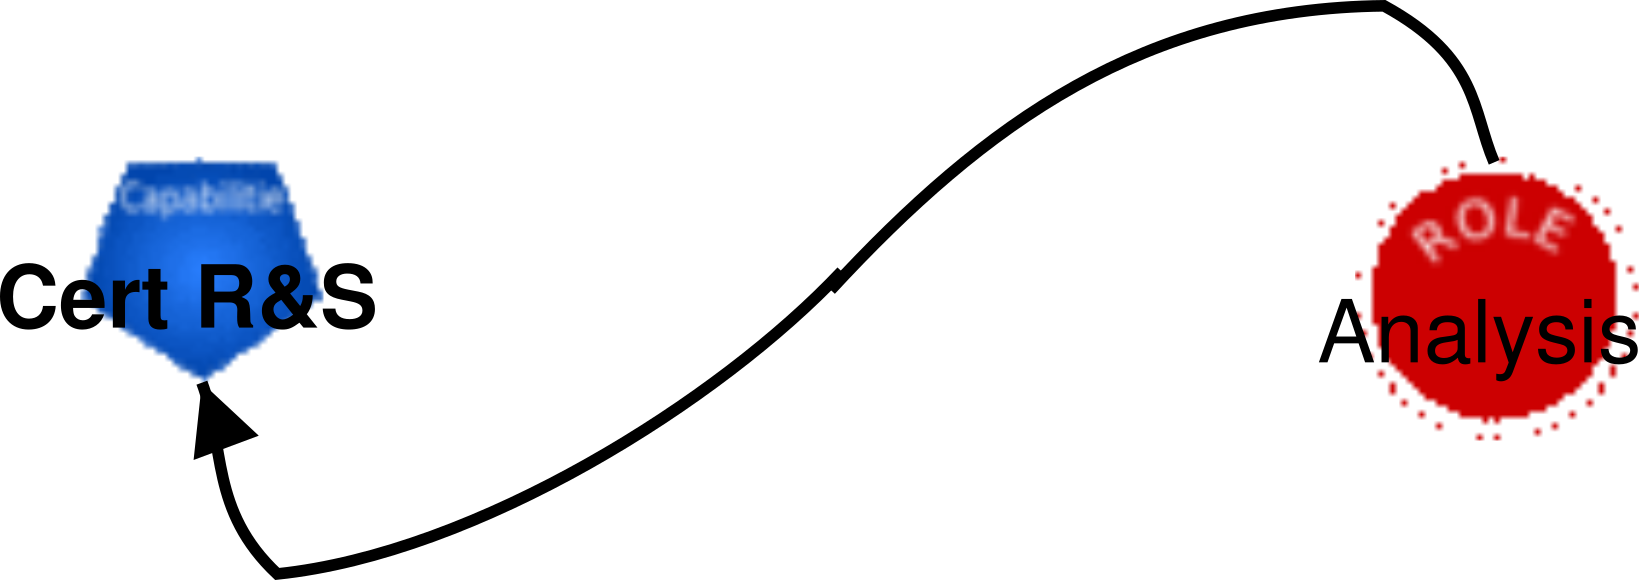
\includegraphics{chapiter1/img/r}
	\caption{\label{fig:The Requirment Relation}The Requirment Relation }
\end{figure}



\subsubsection{Possesses}
In order to determine if some agent has the appropriate set of capabilities to play a given role, OMACS defines a similar relation, the possesses relation, that captures the capabilities a specific agents actually possesses. [4-OMACS]

The possesses relation is formally captured as a function over agents and capabilities that returns a value in the range of 0 to 1,

 possesses: A $\times$ C $\rightarrow$ [0..1]. The real value returned by the possesses function indicates the quality of each capability possessed by the agent; 0 indicates no capability while a 1 indicates a high quality capability. [4-OMACS]


\begin{figure}[th]
	\centering
		
\includegraphics{chapiter1/img/p}
	\caption{\label{fig:Possesses Relation}Possesses Relation }
\end{figure}


\subsubsection{Capable}
Using the capabilities required by a particular role and capabilities possessed by a given agent, we can compute the ability of an agent to play a given role, which we capture in the capable function. The capable function returns a value from 0 to 1 based on how well a given agent may play a specific role, capable: A $\times$ R $\rightarrow$ {[}0..1{]} . [2-OMACS]

Since the capability of an agent, a, to play a specific role  r , application and role specific, OMACS provides the rcf defined in the previous section that controls how this value is computed. Thus, the capable score of an agent playing a particular role is defined via the designer defined rcf of each role.
%#houssam  equation1
\begin{equation}
\forall a:A\textrm{ r:R }capable(a,r)=r.rcf(a)\label{eq:Funccapable}
\end{equation}
While the rcf is user defined, it must conform to one OMACS constraint. 
To be capable of playing a given role in the current organization,
 an agent must possess all the capabilities that are required by that role . [2-OMACS]
%equation2 
\begin{equation}
\text{\ensuremath{\forall}}a:A,r:Rcapable(a,r)>0\text{\ensuremath{\Leftrightarrow}}requires(r)\text{\ensuremath{\subseteq}}{c|possesses(a,c)>0}\label{eq:FuncCapable2}
\end{equation}



\begin{figure}[th]
	\centering
		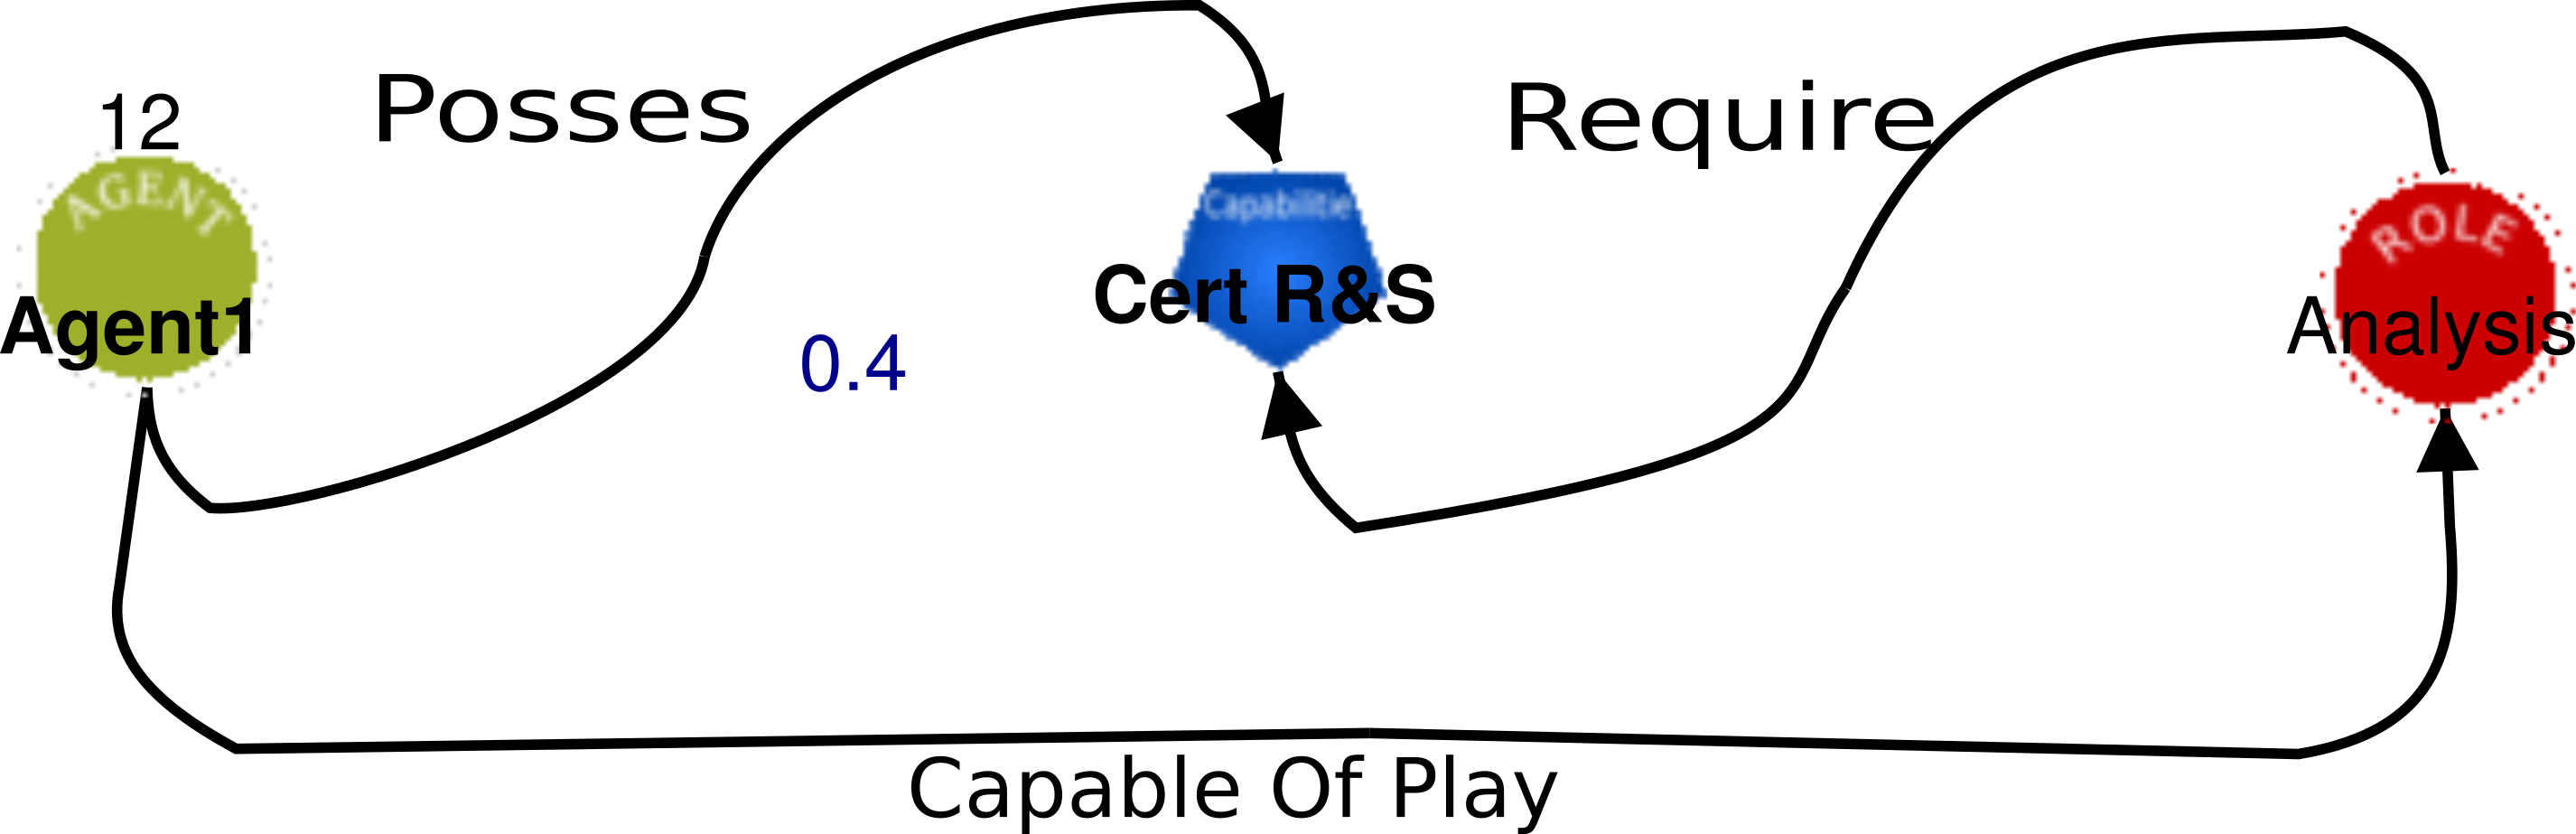
\includegraphics{chapiter1/img/c}
	\caption{\label{fig:Capable Of playing Relation} Agent Capable of Playing Analysis Role}
\end{figure}

\pagebreak


The main goal of OMACS is to provide a mechanism to assign goals to agents [2-OMACS]

in such a way that agents cooperate toward achieving some top-level goal.
Intuitively, this mechanism should provide a way to assign the best agents 
to play the best roles in order to achieve these goals. 

Thus, OMACS has defined  a potential function that captures the ability of an agent 
to play a role in order  to achieve a specific goal.   [2-OMACS]


\subsubsection{Potential}
The potential function maps each agent-role-goal tuple to a real value ranging from 0 to 1, 
potential: A $\times$ R $\times$ G $\rightarrow$ [0..1].[4-OMACS]

Here, a 0 indicates that the agent-role-goal tuple cannot be
used to achieve the goal while a non-zero value indicates how well an agent can play
a specific role in order to achieve a goal.  

The potential of agent a to play role r 
to achieve goal g is defined by combining the capable and achieves functions.[4-OMACS]

\begin{equation}
\forall a:A\textrm{ r:R g:G }potential(a,r,g)=achieves(r,g)*capable(a,r)\label{eq:potentialFunc}
\end{equation}







































%this section should you read it more and reOrgnize 
\section{ Organization \& Reorganization Dynamic System}
 
The constraints above define the legality of the organization structure and its instances.  However,we are also interested in whether or not an assignment of agents to roles satisfying all the organizational policies exists that can allow the system to achieve its goals, which we refer to as organizational viability. [2-OMACS]

Although an organization may be structurally valid, there is no guarantee that an instance of that organization exists that can achieve its goals. 

In actuality, we can never guarantee that the system will ever achieve all its goals due to the dynamic nature of the environment in which the organization operates. To achieve the organizational goals, the system must have the right mix of agents to play the right roles to achieve those goals. 

Essentially, a viable organization is a valid organization that has been populated with the right types and numbers of agents so that it might potentially achieve its goals. [2-OMACS]

\subsection{ Organization and Reorganization }
Each organization has an implicitly defined organization transition function 
that describes how the organization may transition from one organizational state 
to another over the lifetime of the organization.  [2-OMACS]
	
Since agents in an organization as well as their individual capabilities may change over time, 
this function cannot be predefined, but must be computed based on the current state, 
the goal set, G, and the current policies. In our present research with purely autonomous systems, we have only considered reorganization that involves the state of the organization. 

However, we have defined two distinct types of reorganization: state reorganization, which only allows the modification of the organization state, and structure reorganization, which allows modification  of the organization structure (and may require state reorganization to keep the organization consistent).

We define the state of the organization as the set of agents, A, the possesses, capable, and potential functions, and the assignment set, $\varphi$. However, not all these components may actually be under the control of the organization. For our purposes, we assume that agents may enter or leave organizations or relationships, but that these actions are triggers that cause reorganizations and are not the result of reorganizations. 

Likewise, possesses (and thus capable and potential as well) is an automatic calculation that determines the possible assignments of agents to roles and goals in the organization. The calculation of possesses is the only calculation totally controlled by the agent; the organization can only use this information in deciding how to make assignments. This leaves one element that can be modified via state reorganization: $\varphi$.
	[2-OMACS]
\subsubsection{ Goal Set Changes }
Any change in G may cause reorganization. There are three basic types 
of events that can cause achange in G: 
\begin{enumerate}
\item   insertion of a new goal  
\item   goal achievement 
\item   goal failure
\end{enumerate}

is discussed below. 

The first situation deals with new goals being added to G. However, [2-OMACS]
we cannot say with certainty that reorganization will occur based on a new goal in G. 

It is possible that the organization will choose to forego reorganization for a number of reasons, the most likely being that it has simply chosen not to pursue any new goals added to G at the present time.

The second case deals with goal achievement. When a goal g is achieved, G is changed to reflect that event by 

\begin{itemize}
\item  removing g from G
\item  possibly adding new goals
\end{itemize}	

 which are enabled by the achievement of g, into G. Obviously, the agent assigned to achieve goal g is now free to pursue other goals. 

The third instance involves goal failure, which really has two forms: agent-goal failure and goal failure.

When a specific agent cannot achieve goal g but g might still be achievable by some other agent, 
agent-goal failure occurs. 

When agent-goal failure occurs, reorganization must occur to allow the organization to 

\begin{itemize}
\item  choose another agent to achieve g
\item  not pursue g at the current time
\item  choose another goal to pursue instead of g
\end{itemize}	
 
In any of these situations, g is not removed from G since it has not been achieved. In the case where the organization or the environment has changed such that a goal g can never be achieved, then goal failure occurs. 

In this case, g is removed from G and the organization must attempt to assess whether it can still achieve the overall system goals. Reorganization may occur to see if the agent assigned to achieve g can be used elsewhere. 

In all cases, the selection of the appropriate strategy is left to the organization. [2-OMACS]

\subsubsection{Agent Changes }
The second type of change that triggers reorganizations are changes to the set of agents, A, or their individual capabilities.[2-OMACS]

When an agent that is part of $\varphi$ is removed from the organization, a reorganization must occur, even if only to remove the agent and its assignment(s) in $\varphi$. Likewise,when an agent that is part of $\varphi$ loses a capability that negates its ability to play a role that it is assigned, reorganization must occur as well. 

In general, when changes occur in an agent?s capability, reorganization may or may not be necessary, based on the agents capable relation. 

We have identified four specific types of changes in an agents capabilities that may indicate a need for reorganization: 

\begin{enumerate}
\item 
	when an agent gains the ability to play a new role
\item
	when an agent loses the ability to play a role
\item
	when an agent increases its ability to play a specific role
\item
	when an agent decreases its ability to play a specific role.
\end{enumerate}	
 
While case 2 requires reorganization if the agent is currently assigned to play the role for which it no longer has the capability to play, whether or not to reorganize is left up to theorganization when the other three cases (along with 2 when the agent is not currently assigned that role) occur. [2-OMACS]


\subsection{ Reorganization }
Reorganization is the process of changing the assignments of agents to roles to goals as specified
in $\varphi$.  [2-OMACS]

The organization?s oaf function is used to determine the best new $\varphi$; however, total
reorganization may not be necessary or efficient. (In the absence of any information or policies,
an optimal total reorganization would take on the order of 2 A$\times$G$\times$R .)

One approach is to take a local view, in which the organization looks at the OMACS state and
reorganizes in a locally optimal fashion (i.e. hill climbing).
However, when dealing with dynamic environments, it is often desirable to reorganize so that 
the team can operate more efficiently or
effectively in its present situation as well as being adaptable to its changing environment. 

Thus, we would like to take a long-range or global view. Unfortunately, it has been shown that in the
general case globally optimal reorganizations are NEXP-complete and, thus impractical for most
applications with any time constraints . 

Therefore, OMACS provides a mechanism for augmenting the locally optimal algorithm with application specific rules in an attempt to make
reasoning more efficient and to enable globally better solutions.
[2-OMACS]
\subsubsection{ General Purpose Reorganization Examples }

For general-purpose reorganization, the Developers have developed several reorganization algorithms that
give us a default reorganization capability. When a reorganization trigger occurs, general-purpose
reorganization algorithms can be used to find appropriate assignments to achieve the
organizations goals, if possible. [2-OMACS]

To compute the best reorganization, an algorithm that simply
optimizes the organizations oaf might seem appropriate; however, this approach is short sighted.
First, it does not deal with the cost associated with reorganizing and, second, it does not consider
the reason reorganizing was initially undertaken. Exploiting reorganizing costs requires a
distributed solution since the cost for robots to change roles is not globally known. 

For instance, if an agent is required to perform a complex computation, any effort toward that computation
would be lost if the agent was reassigned to another role/goal Considering the reason for
reorganization may enable less extensive (and less costly) reorganization. If the reason for
reorganizing is to fill a single role, then a total reorganization may be a waste of time and
resources. [2-OMACS]

\pagebreak

\section{Conclusion}

This chapter describes how to design adaptive multiagent
systems using an organizational model, which defines the
entities and relationships of a typical organization.

 The major elements of the model consist of goals, roles, agents,
capabilities, and the relationships between them. By
designing a system using the model, and we focus on OMACS framework
because it handeling reorganization system more then other framework

In the following chapter will discuss other model
we can use it to modeling the multi-Agent System
\textbf{}

 
%
\chapter*{General Conclusion}

\addcontentsline{toc}{chapter}{\numberline{}{Conclusion Générale}}

Through this paper, we saw out objective was to optimise a multi agent system 
and this MaS represented according the OMACS framework .

We have introduce  in the first chapter the definition of elements and the relation between these element in OMACS .

The Second chapter was the  PGraph Framework and  Process Network Synthesis , the basic concept and mathematical definition  of this framework , and i mention 
three algorithm applicable on PNS 

in the Third chapter , we presented our approach for transforam MaS in OMACS presentation into PNS Model , we start with defining the meta model for both framework i use ( OMACS and PNS )  followed by an overview about the Tool $AToM^3$ that tool allow us to define the meta model and generate a formalism 
from these meta model , and use formalism to create ot modelise you own model  .

the next step it is to define a graph grammar that allows to transform from source graph in this case is OMACS model into target graph (PNS model) , after execute this transforamtion we can not be used directly for optimisation with the existing tools , for thsi we have to propose another approach to transforam 
the model in PNS into xml file .

Now we can import the xml file into the PGraph-Studio and apply the Algorithm 
of optimisation . 


\backmatter
\pagestyle{plain}

\phantomsection
\addcontentsline{toc}{chapter}{\numberline{}{Bibliographie}}

\bibliographystyle{ieeetr}
%\bibliography{biblo}




\appendix

\setcounter{figure}{0}

%\include{anneX1} 	
\end{document}


